% %
% main.tex
%

% notes = hide | show | only
\documentclass[xcolor=dvipsnames,dvip,notes=show,table]{beamer}

% Para crear una versión 'handout' (impresa)
%\documentclass[xcolor=pst,dvips,handout,notes=show]{beamer}

%
% cabeceras.tex
%

\usepackage[T1]{fontenc}

 \definecolor{ZurichBlue}{rgb}{.255,.41,.884}
 \beamertemplateshadingbackground{white!10}{white!10}
%\usepackage{beamerthemeWarsaw}

% \usepackage{longtable}
\usepackage{beamerthemeBoadilla}


%\usepackage{tikz,times}
\usetheme{boxes}
%\usepackage{handoutWithNotes}
\usepackage{pgfpages}
%\pgfpagesuselayout{2 on 1}[a4paper,border shrink=5mm]


%\usecolortheme[named=OliveGreen]{structure} 
\setbeamertemplate{items}[ball] 
%\setbeamertemplate{blocks}[rounded][shadow=true] 
\setbeamertemplate{footline}[page number]
\addtocounter{framenumber}{-1}
%Handout



%\usepackage{beamertheme}
%\usepackage{beamerthemeshadow}
\useoutertheme[hooks]{tree}
 
% \setbeamertemplate{headline}[default] % The default is just an empty headline.
% \setbeamertemplate{headline}[infolines theme]
% \setbeamertemplate{headline}[miniframes theme]
% \setbeamertemplate{headline}[sidebar theme]
% \setbeamertemplate{headline}[smoothtree theme]
% \setbeamertemplate{headline}[smoothbars theme]
% \setbeamertemplate{headline}[tree]
\beamertemplatetransparentcovereddynamic
% spanish
\usepackage[spanish]{babel}
\usepackage[utf8]{inputenc}

% diagramas
%\usepackage{pst-eps,epstopdf}
\usepackage{pst-node}
%\usepackage{pst-all}
\usepackage{pst-blur}
%\usepackage{pst-tree}

% incrustaciones de código fuente
\usepackage{listings}

% matemáticas y símbolos
\usepackage{amsmath}
\usepackage{amssymb}
\usepackage[right]{eurosym}
\usepackage{ulem}

% colores
\usepackage{colortbl}

%\usepackage{algorithm2e}
%\usepackage{algorithm}
%\usepackage{algorithmic}

\lstset{language=[90]Fortran,
  basicstyle=\ttfamily,
  keywordstyle=\color{darkred},
  commentstyle=\color{green},
  frame=trBL,
  stringstyle=\color{violet},
  frameround=tttt,
  backgroundcolor=\color{lightyellow},
  morecomment=[l]{!\ }% Comment only with space after !
}


% 
% \lstset{%
%   language=Fortran,
% 	basicstyle=\footnotesize\sffamily,
% 	keywordstyle=\color{darkred}
%  	stringstyle=\color{violet}
%  	commentstyle=\color{blue}
%  	showspaces=false,
%  	showtabs=false,
%  	showstringspaces=false,
%  	frame=trBL,
%         frameround=tttt,
%         backgroundcolor=\color{lightyellow},
%  	extendedchars=true,
%  	numbers=none,
%         aboveskip=0.5cm,
%         belowskip=0.5cm,
%         xleftmargin=1cm,
%         xrightmargin=1cm,
% 	breaklines=true
% }
\definecolor{darkred}{rgb}{0.5, 0, 0}
\definecolor{violet}{rgb}{1, 0, 1}
\definecolor{lightyellow}{rgb}{1,1,0.8}


\usepackage{latexsym}
\usepackage{amsmath}
\usepackage{amssymb}
\usepackage{amsthm}

\usepackage{xspace}



\hyphenation{real}

\newrgbcolor{ColorEncabezadoTabla}{0.7 0.7 0.9}
\newrgbcolor{ColorFila1}{0.8 0.8 0.7}
\newrgbcolor{ColorFila2}{0.8 0.7 0.8}
\newrgbcolor{ColorTotal}{0.7 0.9 0.7}


% \usepackage{tikz,times}
% \usetikzlibrary{mindmap,backgrounds}
\usepackage{multirow}


%%%%%%%%%%%%%%%%%%%%%%%%%%%%%%%%%%%%%%%%%%%%%%%%%%%%%%%%%%%%%%%%%%%%%%

\title[The CORFU technique | MTSR 2013]{Towards a stepwise method for unifying and reconciling corporate names in public contracts metadata. \\ The CORFU technique.}
\author[Jose María Álvarez Rodríguez]{\textbf{Michalis Vafopoulos} (speaker) \\ and \\ \{Jose María Álvarez-Rodríguez, Patricia Ordoñez De Pablos and \\ Jose Emilio Labra-Gayo\}}
\institute{MTSR 2013 | 7th Metadata and Semantics Research Conference \\ Track on Metadata and Semantics for Open Repositories, Research Information Systems and Data Infrastructures}


\date{}

\begin{document}

\frame{
\titlepage

}

\frame{
\tableofcontents

}


\section{Introduction}

\frame{
  \frametitle{The Problem...What is the ``Big Name''?} 
  
\begin{table}[!htb]
\renewcommand{\arraystretch}{1.3}
\tiny
\begin{center}
\begin{tabular}{|p{7cm}|p{2cm}|}
\hline
  ``Oracle (Corp) Aust Pty Ltd''  & \multirow{11}{*}{``Oracle''} \\
 ``Oracle Corp (Aust) Pty Ltd''  &  \\
  ``Oracle Corp Aust Pty Ltd'' & \\
  ``Oracle Corp. Australia'' & \\
  ``Oracle Corp. Australia Pty.Ltd.'' & \\
  ``Oracle Corpoartion (Aust) Pty Ltd'' & \\
  ``Oracle Corporate Aust Pty Ltd'' & \\
  ``Oracle Corporation'' & \\
  ``Oracle Risk Consultants'' & \\
  ``ORACLE SYSTEMS (AUSTRALIA) PTY LTD'' & \\
  ``Oracle University''  & \\ 
  \ldots  & \\ \hline
   ``Accenture'' & \multirow{8}{*}{``Accenture''} \\
  ``Accenture Aust Holdings'' &  \\ 
   ``Accenture Aust Holdings'' & \\  
   ``Accenture Aust Holdings Pty Ltd'' & \\
   ``Accenture  Australia Holding P/L'' & \\
   ``Accenture Australia Holdings P/Ltd'' & \\
   ``Accenture Australia Holdings Pty Lt''  & \\  
  ``Accenture Australia Limited'' & \\
  \ldots  & \\ \hline
  \ldots & \ldots \\
  
  \hline
  \end{tabular}
\end{center}
\end{table} 

}

\frame{
  \frametitle{...and if you have 400K corporate names} 
    \begin{figure}[!htb]
\centering
 
\includegraphics[width=9cm]{imgs/corfu-init}
\end{figure}
  
  }
  
  
\frame{
  \frametitle{Scope}
  
  \begin{block}{Public Procurement}<1->
   \begin{enumerate}
    \item e-Procurement is a strategic sector (17\% of the GDP in Europe).
    \item Action Plans 2004 and 2020.
    \item Projects: E-Certis, Fiscalis 2013, E-Prior, PEPPOL, STORK,etc.
    \item Other actions: TED, RAMON metadata server, CPV, NUTS, etc.
    \item Legal Framework.
    \item Boost participation with special focus on SMEs.s
   \end{enumerate}
  \end{block}

   \begin{alertblock}{...but it also requires...}<2->
   \begin{enumerate}
    \item Accomplish with Open Data principles.
    \item Improve transparency of public bodies.
    \item Track where public money goes.
    \item \ldots
   \end{enumerate}
  \end{alertblock}
  
  
  }
  
\frame{
  \frametitle{The Problem...}
  
  \begin{block}{How can we track public procurement processes?}<1->
   \begin{enumerate}
    \item Data and information is already out there.
    \item Relevant metadata can be (re)used:
    \begin{itemize}
     \item Normalized product scheme classifications such as the CPV 2008 (Common Procurement Vocabulary)~\cite{AlvarezRodrguez2013}.
     \item Territorial units (NUTS).
     \item Currency.
    \end{itemize}
    \item \ldots
   \end{enumerate}
  \end{block}
  
\begin{alertblock}{...and ``names''?}<2->
  Both \textbf{Payer} and \textbf{Payee} names are not usually normalized.
\end{alertblock}
  

\begin{block}{Normalized and unified names (``Big Name'')...}<3->
  ...with the aim of tracking both payers and payees.
\end{block}
   
  }

   
\frame{
  \frametitle{The Problem...}
  \begin{block}{Some remarks...}
   \begin{enumerate}
    \item It is \textbf{not} a mere problem of reconciling entities (dealing with)...
    \begin{itemize}
     \item Misspelling errors.
     \item Name/acronym mismatches.
     \item ...
    \end{itemize}
    \item ...but to \textbf{create a unique name or link }($n$ string literals $\to$ $1$ company $\to$ $1$ URI). 
    \item E.g.
    \begin{itemize}
     \item  ``Oracle'' and ``Oracle University'' could be respectively aligned to the entities $<$Oracle\_Corporation$>$ and $<$Oracle\_University$>$
     \item ...but the problem of grouping by a unique (\textit{Big}) name, identifier or resource still remains. 
    \end{itemize}
   \end{enumerate}

  \end{block}

  }

     
\frame{
  \frametitle{The Public Spending initiative...}
    
\begin{columns}[c] % the "c" option specifies center vertical alignment
\column{.5\textwidth} % column designated by a command


\begin{exampleblock}{...a joint effort trying to answer...}
\scriptsize
 \begin{enumerate}
\item Who really gets the public money?
\item  For what? From whom?
\item  Can we compare them?
\item  Is public spending effective?
\item  \ldots
\end{enumerate}
\end{exampleblock}


\column{.5\textwidth}


\begin{figure}[htb]
\centering
	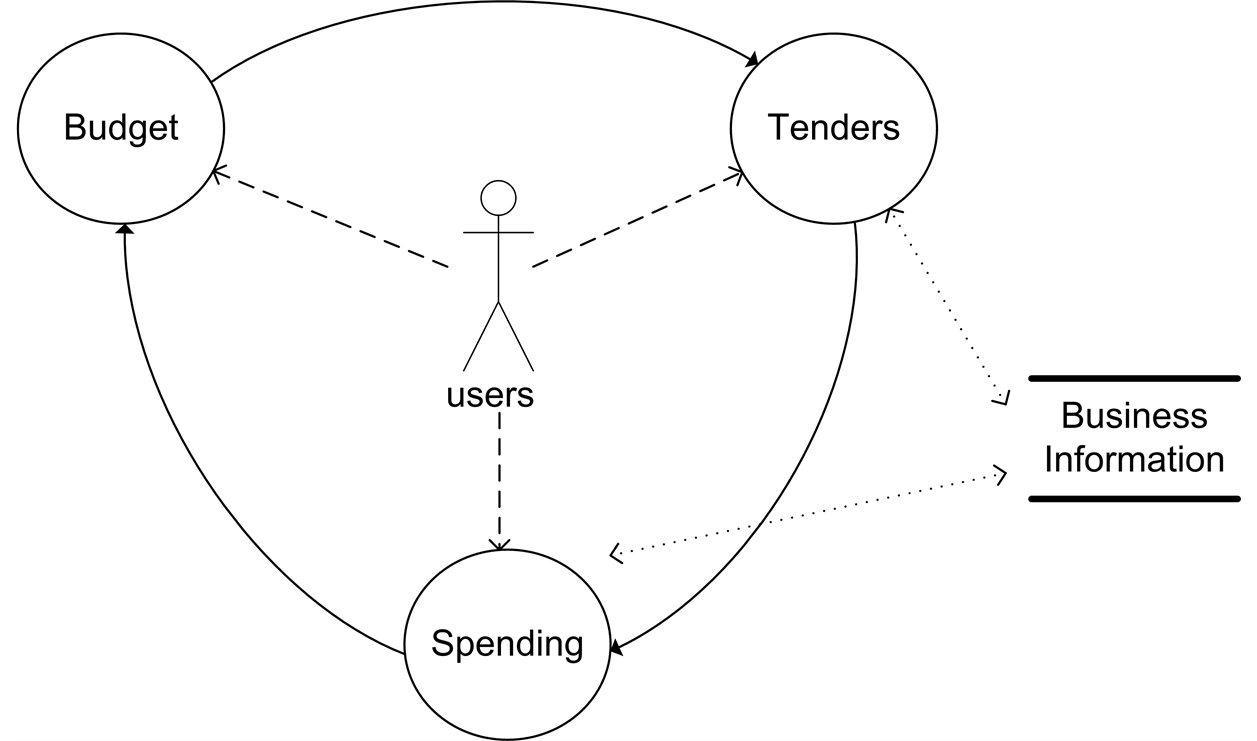
\includegraphics[width=6cm]{imgs/public-budget}
%\caption{Modelo $5\star$ (W3C).}
\end{figure}

\end{columns}

Learn more: \url{http://publicspending.net/}

  
  }
\section{Related Work}

\frame{
  \frametitle{Natural Language Processing, Computational Linguistics and Entity Reconciliation.} 
  \scriptsize
  \begin{block}{Existing works and APIs to deal with natural language issues}<1->
  \begin{enumerate}
 \item Misspelling errors~\cite{NorvigSpelling,StanfordSpelling}.
 \item Name/acronym mismatches~\cite{Yeates99automaticextraction}.
 \item APIs such as NLTK for Python, Lingpipe, OpenNLP or Gate for Java and search engines such as Apache Lucene/Solr.
 \item Extraction of clinical terms~\cite{Wang:2009:ARN:1667884.1667888} for electronic health records.
 \item Creation of bibliometrics~\cite{Galvez2006} or identification of gene names~\cite{Krauthammer:2004:TIB:1053007.1053018,Galvez2012}.
 \item Entity reconciliation processes~\cite{DBLP:conf/semweb/IseleJB10,Serimi} using the DBPedia~\cite{Mendes:2011:DSS:2063518.2063519} or URI comparison~\cite{conf/www/MaaliCP11}.
 \item Tools such as Google Refine, etc. 
 \end{enumerate}
\end{block}

  
 \begin{alertblock}{Preliminary evaluation...}<2->
  \begin{itemize}
   \item Algorithms to deal with natural language heterogeneities are already available.
   \item Existing works are usually focused in some domain (prototypes cannot be easily customized to other domain).
   \item ...but methodologies and NLP algorithms can be re-applied to new domains.
  \end{itemize}

 \end{alertblock}

 
 
}


\frame{
  \frametitle{Corporate Information.} 
  \scriptsize
  \begin{block}{Corporate Databases}<1->
  \begin{enumerate}
 \item Some corporate databases: The Spanish Chambers of Commerce, ``Empresia.es'' or ``Axesor.es'' to name a few (just in Spain).
 \item The DBPedia and the Orgpedia~\cite{Orgpedia}.
 \item The CrocTail~\cite{croctail} effort (part of the ``Corporate Research Project'').
 \item ``The Open Database Of The Corporate World''~\cite{Opencorporates}.
 \item Forbes, Google Places, Google Maps, Foursquare, Linkedin Companies or Facebook.
 \item Similar initiatives: Openspending.net, LOD2 project e-Procurement, etc.
 \item \ldots
 \end{enumerate}
\end{block}

  
 \begin{alertblock}{Preliminary evaluation...}<2->
  \begin{itemize}
   \item Corporate information is public but access is restricted or under a fee (valuable metadata)...
   \item Large databases (``infobesity?'') but...
   \item ...the problem of mapping ,($n$ string literals $\to$ $1$ company $\to$ $1$ URI) as a human would do, still remains.
  \end{itemize}

 \end{alertblock}
 
}




\section{The CORFU technique}

\frame{
  \frametitle{Company, ORganization and Firm name Unifier-CORFU (I)}
  
    \begin{figure}[!htb]
\centering
 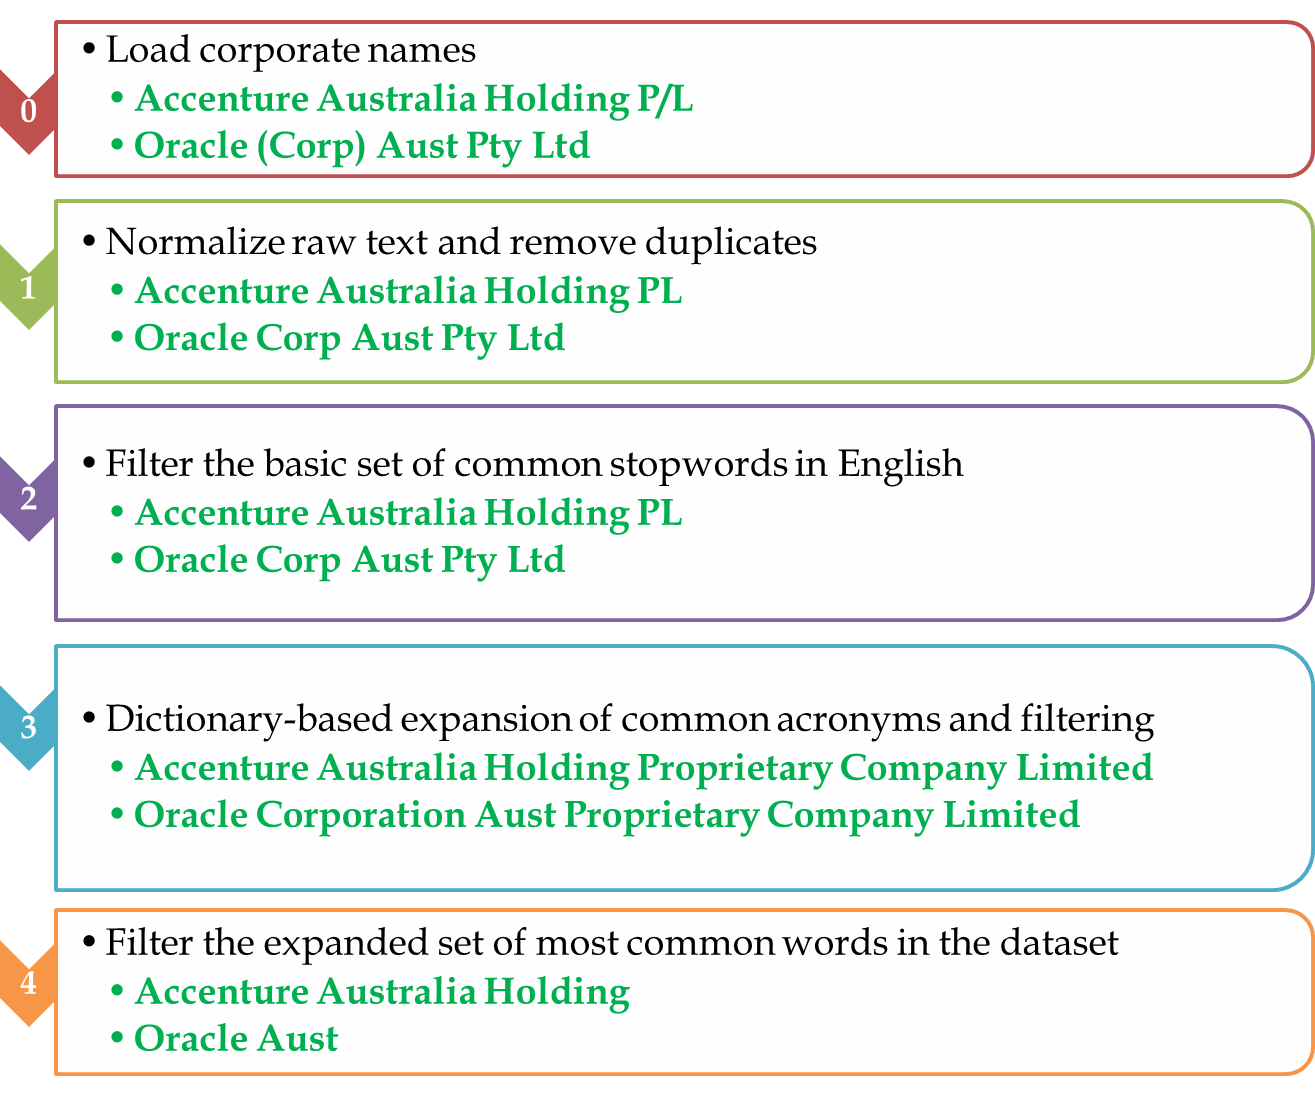
\includegraphics[width=9cm]{imgs/corfu-flow-1}
\end{figure}



}

\frame{
  \frametitle{Company, ORganization and Firm name Unifier-CORFU (II)}
  
    \begin{figure}[!htb]
\centering
 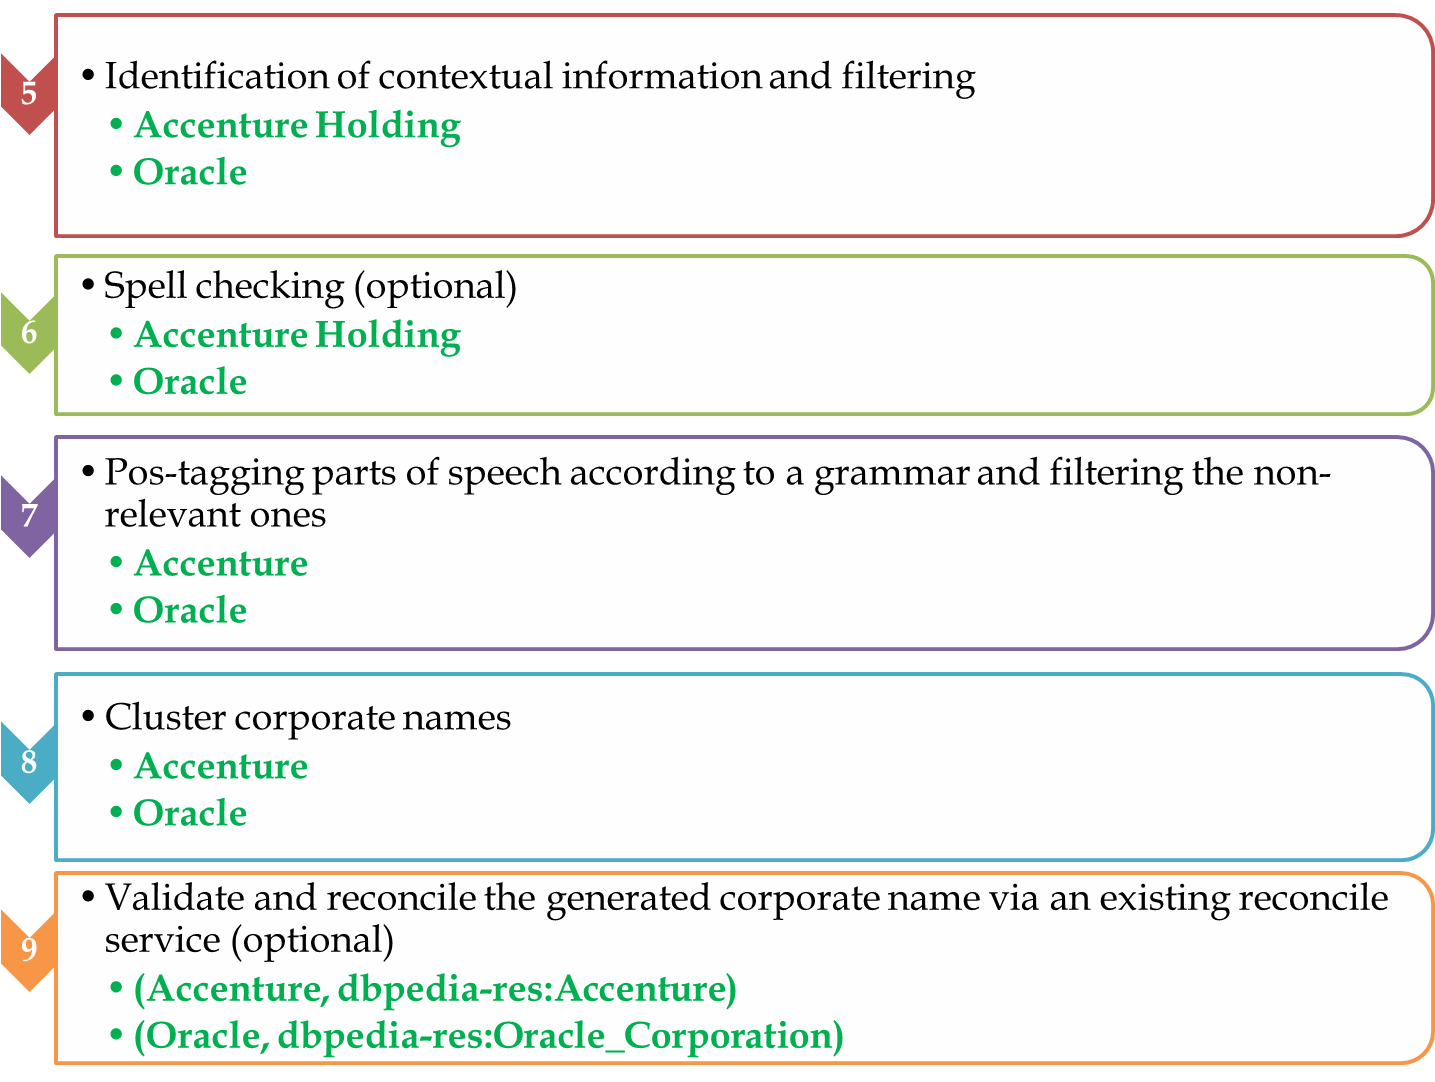
\includegraphics[width=9cm]{imgs/corfu-flow-2}
\end{figure}



}



\frame{
  \frametitle{Example step by step...}
  \begin{itemize}
   \item Scenario: Australian supplier names (400K).
   \item $1^{st}$ try: use of Google Refine+Open Corporates reconciliation service (just an 8\% of unified names, see Figure below).
   \item $2^{nd}$ try: design of the \textbf{CORFU} technique using Python NLTK and other third-party APIs for NLP processing.
  \end{itemize}

  
\begin{figure}[htb]
\centering
	
\includegraphics[width=4cm]{imgs/previous-corfu}
%\caption{Modelo $5\star$ (W3C).}
\end{figure}

  
}

\frame{
  \frametitle{Step 0: Load corporate names} 
  \begin{block}{Load}
   \begin{description}
    \item [Input:] a list of corporate names as raw text (one per line).
    \item [Output:] a set of names represented as strings.
    \item [Example:] 
    \begin{itemize} \item  ``Accenture  Australia Holding P/L'' \item  ``Oracle (Corp) Aust Pty Ltd''  \end{itemize} 
   \end{description}

  \end{block}

}



\frame{
  \frametitle{Step 1: Normalize raw text and remove duplicates} 
  \begin{exampleblock}{Normalize}
   \begin{description}
    \item [Input:] a set of names represented as strings.
    \item [Process:] this step is comprised of: 
    \begin{enumerate}
     \item Remove strange characters and punctuation marks but keeping those that are part of a word avoiding potential changes in abbreviations or acronyms;
     \item Lowercase raw text (although some semantics can be lost previous works and empirical tests show that this is the best approach).
     \item Remove duplicates.
     \item Lemmatize the corporate name. 
    \end{enumerate}
    \item [Output:] a set of normalized corporate names.
    \item [Example:] 
    \begin{itemize} \item  ``Accenture  Australia Holding PL'' \item  ``Oracle Corp Aust Pty Ltd'' \end{itemize}
    
   \end{description}

  \end{exampleblock}

}

\frame{
  \frametitle{Step 2: Filter the basic set of common stopwords in English} 
  \begin{alertblock}{Filter}
   \begin{description}
    \item [Input:] a set of normalized corporate names and a set of stopwords.
    \item [Process:] load a set of stopwords (a minimal set of stopwords from the Python NLTK API has been used):
    \begin{itemize}
     \item Including common English stopwords but...
     \item Avoiding to filter relevant words.
    \end{itemize}
  
    \item [Output:] a set of cleaned and normalized corporate names.
    \item [Example:] 
   \begin{itemize} \item  ``Accenture  Australia Holding PL'' \item  ``Oracle Corp Aust Pty Ltd'' \end{itemize}
   \end{description}

  \end{alertblock}

}


\frame{
  \frametitle{Step 3: Dictionary-based expansion of common acronyms and filtering} 
  \begin{block}{Dictionary-based expansion}
   \begin{description}
    \item [Input:]  a set of cleaned and normalized corporate names and a dictionary of acronyms.
    \item [Process:] load the dictionary of acronyms and expand.
    \item [Output:] a set of cleaned, normalized and acronym-expanded corporate names.
    \item [Example:] 
    \begin{itemize} \item  ``Accenture  Australia Holding Proprietary Company Limited'' \item  ``Oracle Corporation Aust Proprietary Company Limited'' \end{itemize}
   \end{description}

  \end{block}

}
 

\frame{
  \frametitle{Step 4: Filter the expanded set of most common words in the dataset} 
  \begin{exampleblock}{Filter}
   \begin{description}
    \item [Input:] a set of cleaned, normalized and acronym-expanded corporate names.
    \item [Process:] extract statistics of ``most used words'' in the input dataset, expand those words and filter.
    \item [Output:] a set of cleaned, normalized and acronym-expanded corporate names.
    \item [Example:] 
    \begin{itemize} \item  ``Accenture  Australia Holding'' \item  ``Oracle Aust'' \end{itemize}
  \end{description}

  \end{exampleblock}

}

\frame{
  \frametitle{Step 5: Identification of contextual information and filtering } 
  \begin{alertblock}{Context filtering}
   \begin{description}
    \item [Input:] a set of cleaned, normalized and acronym-expanded corporate names.
    \item [Output:] a set of cleaned, normalized and acronym-expanded corporate names without contextual information.
    \item [Example:] 
    \begin{itemize} \item  ``Accenture Holding'' \item  ``Oracle'' \end{itemize}
  \end{description}

  \end{alertblock}

}


\frame{
  \frametitle{Step 6: Spell checking (optional)} 
  \begin{block}{Spell checking}
   \begin{description}
    \item [Input:] a set of cleaned, normalized and acronym-expanded corporate names without contextual information.
    \item [Output:] the previous set without spelling errors.
    \item [Example:] 
    \begin{itemize} \item  ``Accenture Holding'' \item  ``Oracle'' \end{itemize}
  \end{description}

  \end{block}

}


\frame{
  \frametitle{Step 7: Pos-tagging parts of speech according to a grammar and filtering the non-relevant ones } 
  \begin{exampleblock}{Pos-tagging}
   \begin{description}
    \item [Input:] a set of cleaned, normalized and acronym-expanded corporate names without contextual information.
    \item [Output:] a tree according to a pre-defined grammar for corporate names that only contains nouns.
    \item [Example:] 
    \begin{itemize}  \item  ``Accenture'' \item  ``Oracle'' \end{itemize}
  \end{description}

  \end{exampleblock}

}


\frame{
  \frametitle{Step 8: Cluster corporate names} 
  \begin{alertblock}{Clustering}
   \begin{description}
    \item [Input:] a set of strings derivate from the aforementioned tree.
    \item [Output:] a set of clusters for each extracted corporate name.
    \item [Example:] 
    \begin{itemize}  \item  ``Accenture'' \item  ``Oracle'' \end{itemize}
  \end{description}

  \end{alertblock}

}


\frame{
  \frametitle{Step 9: Validate and reconcile the generated corporate name via an existing reconcile service (optional)} 
  \begin{block}{Validate and reconcile}
   \begin{description}
    \item [Input:] a set of clusters for each extracted corporate name.
    \item [Output:] ($n$ string literals $\to$ $1$ company $\to$ $1$ URI). 
    \item [Example:] 
   \begin{itemize}  \item  (``Accenture'', dbpedia-res:Accenture) \item  (``Oracle'', dbpedia-res:Oracle\_Corporation) \end{itemize}
  \end{description}

  \end{block}

}

\begin{frame}[fragile]

  \frametitle{Representing and querying the corporate information in RDF...} 
\tiny
\begin{lstlisting}[language=XML]  
:o1 a org:Organization;
  skos:prefLabel ``Oracle'';
  skos:altLabel  ``Oracle Corporation'',  ``Oracle (Corp)  Aust Pty Ltd'',  ...;
  skos:closeMatch  dbpedia-res: Oracle_Corporation;
   ...
.
\end{lstlisting}

\begin{lstlisting}[language=SQL]  
SELECT  str(?label) (COUNT(?org) as ?pCount) WHERE{
  ?ppn :rewarded-to ?org .
  ?org rdf:type org:Organization.
  ?org skos:prefLabel ?label.
  ...
}
GROUP BY str(?label) 
ORDER BY desc(?pCount)
\end{lstlisting}

\end{frame}

\subsection{Use Case: the Public Spending initiative}

\frame{
  \frametitle{Demo and application...} 
      
  \begin{figure}[!htb]
\centering
 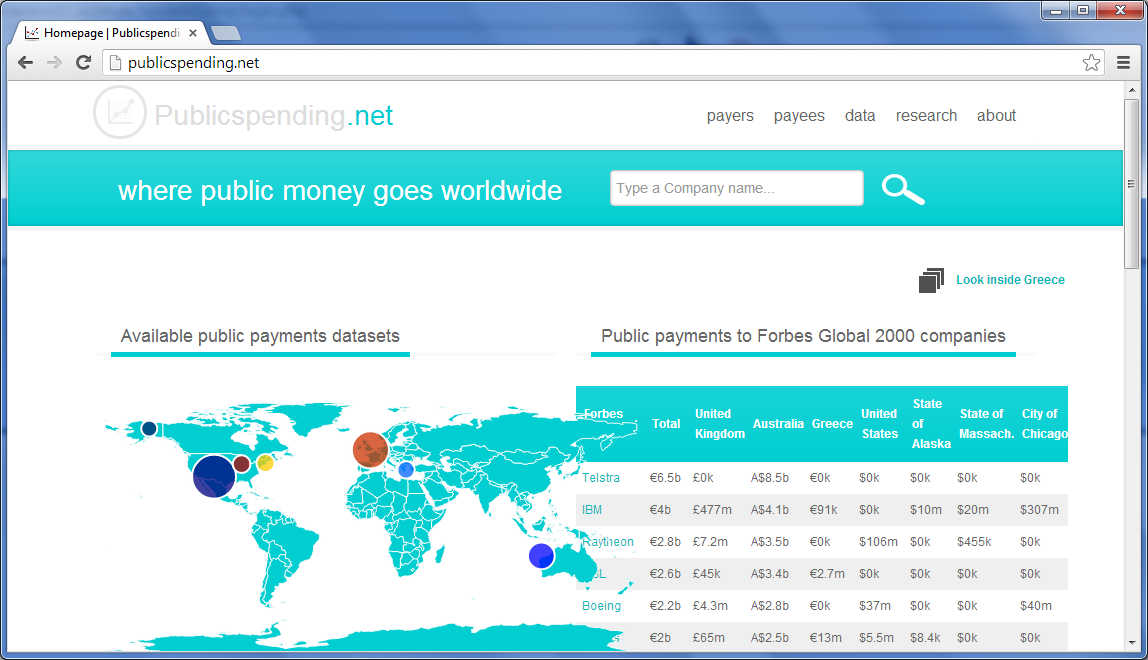
\includegraphics[width=9cm]{imgs/psnet}
\end{figure}
 
 
 Learn more: \url{http://publicspending.net/}
}


\section{Evaluation and Discussion}


\frame{
  \frametitle{The case of Australian supplier names...} 
  
  \begin{table}[!htb]
\renewcommand{\arraystretch}{1.3}
\tiny
\begin{center}
\begin{tabular}{|l|p{4.5cm}|p{4.5cm}|}
\hline
  \textbf{Step} & \textbf{Name} & \textbf{Customization}  \\  \hline
  $0$ & Load corporate names &  $430188$ full names and $77526$ unique names (period 2004-2012) \\ \hline
  $1$ & Normalize raw text and remove duplicates & Default \\ \hline
  $2$ & Filter the basic set of common stopwords in English & Default\\ \hline
  $3$ & Filter the expanded set of most common words in the dataset & Two stopwords sets: $355$ words (manually) and words with more than $n=50 $ apparitions (automatically) \\ \hline
  $4$ & Dictionary-based expansion of common acronyms and filtering & Set of $50$ acronyms variations (manually) \\ \hline
  $5$ & Identification of contextual information and filtering & Use of Geonames REST service\\ \hline
  $6$ & Spell checking (optional) & Train dataset of $128457$ words provided by Peter Norvig's spell-checker~\cite{NorvigSpelling}. \\ \hline
  $7$ & Pos-tagging parts of speech according to a grammar and filtering the non-relevant ones & Default \\ \hline
  $8$ & Cluster corporate names & Default \\ \hline
  $9$ & Validate and reconcile the generated corporate name via an existing reconcile service (optional) & Python client and Google Refine \\ \hline
  \hline
  \end{tabular}
   \label{config-corfu}
  \end{center}
\end{table} 


}



\frame{
  \frametitle{Research Design} 
  
  \begin{enumerate}

   \item Configure and execute the CORFU technique.
   \item Validate (manually) the dump of unified names and calculate: 
   \begin{itemize}
    \item \textbf{Precision}, see Eq.~\ref{eq-1}, is ``the number of supplier names that have been correctly unified under the same name''
    \item \textbf{Recall} is, see Eq.~\ref{eq-2}, ``the number of supplier names that have not been correctly classified under a proper name'' and \textbf{F1} score, see Eq.~\ref{eq-3}, where...
    \item \ldots~$tp$ is ``the number of corporate names \textbf{properly unified}''
    \item \ldots~$fp$ is ``the number of corporate names \textbf{wrongly unified}''
    \item \ldots~$tn$ is ``the number of corporate names \textbf{properly non-unified}'' and 
    \item \ldots~$fn$ is ``the number of corporate names \textbf{wrongly non-unified}''.
   \end{itemize}
  \end{enumerate}

  
  \begin{figure}[ht]
\begin{minipage}[b]{0.45\linewidth}
\centering
\begin{equation}\label{eq-1}
Precision = \frac{tp}{tp+fp} 
\end{equation}
\end{minipage}
\hspace{0.5cm}
\begin{minipage}[b]{0.45\linewidth}
\centering
\begin{equation}\label{eq-2}
Recall = \frac{tp}{tp+fn}
\end{equation}
\end{minipage}
\end{figure}


\begin{equation}\label{eq-3}
F1 = 2 \cdot \frac{Precision \cdot Recall}{ Precision + Recall}
\end{equation}



}

\frame{
  \frametitle{Results of applying the CORFU approach to the Australian supplier names.} 
  
  
\begin{table}[!h]
\renewcommand{\arraystretch}{1.3}
\scriptsize
\begin{center}
\begin{tabular}{|p{1.8cm}|p{1.3cm}|p{1.3cm}|p{1.3cm}|l|l|l|}
\hline
  \textbf{Total number of companies} & \textbf{Unique names}& \textbf{CORFU unified names}& \textbf{\% of unified names} & \textbf{Precision} & \textbf{Recall} & \textbf{F1 score} \\  \hline
   $430188$ & $77526$ & $40277$  &$48\%$ & $0.762$ & $0.311$&$0.441$ \\ \hline   
   $430188$ & $299$ in $77526$ & $68$ & $100\%$&  $0.926$ & $0.926$ &$0.926$\\ \hline
  \hline
  \end{tabular}
  %\caption{Results of applying the CORFU approach to the Australian supplier names.}
  \label{tabla:aus-results}
  \end{center}
\end{table} 

\scriptsize
\begin{exampleblock}{Comments}
 \begin{itemize}
  \item A $48\%$ ($77526-40278=37248$) of supplier names have been unified with a precision of $0.762$ and a recall of $0.311$ (best values must be close to $1$).
  \item The first 100 companies in the Forbes list, actually $68$ companies were found in the dataset with $299$ appearances.
  \item Results~\footnote{Best values must be close to $1$.}, in this second case, show a better performance: precision, $0.926$, and recall, $0.926$.
   \end{itemize}

\end{exampleblock}
 
  }



  

  \frame{
  \frametitle{Graphical view after applying the CORFU technique...}
\begin{figure}[htb]
\centering
	
\includegraphics[width=6cm]{imgs/corfu-stats}
%\caption{Modelo $5\star$ (W3C).}
\end{figure}

  }
  
  
  
  \frame{
  \frametitle{Graphical view after applying the CORFU technique to the first 100 Forbes companies...}
\begin{figure}[htb]
\centering
	
\includegraphics[width=6cm]{imgs/corfu-forbes-100}
%\caption{Modelo $5\star$ (W3C).}
\end{figure}

  }
  
  
    \frame{
  \frametitle{...the first 100 Forbes companies in bubbles...}
\begin{figure}[htb]
\centering
	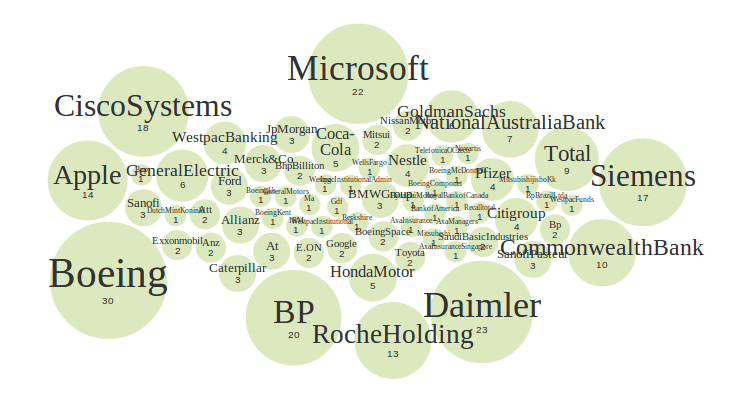
\includegraphics[width=10cm]{imgs/forbes}
%\caption{Modelo $5\star$ (W3C).}
\end{figure}

  }
  
  
  
\frame{
  \frametitle{Discussion} 
  

  \begin{exampleblock}{Advantages}<1->
   \begin{enumerate}
    \item A \textbf{custom} technique for a particular domain.
    \item Unification works pretty nice.
    \item It enables the possibility of comparing companies in public procurement.
   \end{enumerate}

  \end{exampleblock}


    \begin{alertblock}{Drawbacks}<2->
   \begin{enumerate}
    \item Execution time (~20' for Australian corporate names).
    \item It is necessary to test with other datasets.
    \item It requires the use of more advanced data mining techniques for machine learning.
    \item It should be applied to other domains (Bibliometrics?).
   \end{enumerate}

  \end{alertblock}





}

\section{Conclusions and Future Work}

\frame{
  \frametitle{Conclusions} 
  \begin{enumerate}
   \item The public e-Procurement sector is seeking for new methods to: 
   \begin{itemize}
    \item ...improve interoperability
    \item ...boost transparency
    \item ...or increase participation to name a few.
   \end{itemize}
   \item The PublicSpending initiative is addressing some of the challenges in the e-Procurement sector.
   \item The CORFU technique is a key enabler to ease the comparison of countries, payers, payees, etc.
   \item ...a technique that helps to take the most of data.
   \item It must be technically improved and extended to cover more datasets and to be ``smarter''.
  \end{enumerate}

}


\frame{
  \frametitle{Future Work} 
  
   \begin{enumerate}
   \item Application to new public procurement datasets.
   \item Reuse the Opencorporates reconciliation service (it has been updated).
   \item Contribute to the e-Procurement sector and the PublicSpending initiative~\cite{vaf2012,vaf2012a}.
   \item Add more advanced NLP techniques: $n-grams$.
   \item Add machine learning algorithms to automatically classify new corporate names.
   \item Improve the execution time (performance).
   \item ...
  \end{enumerate}
  
}




\section*{End of the presentation...}

\frame{
    
  \begin{figure}[!htb]
\centering
 
\includegraphics[width=9cm]{imgs/thanks}
\end{figure}


}



\section{Metadata and Information}


\frame{
  \frametitle{Acknowledgements...} 
 \scriptsize
   \begin{table}[!htb]
  \begin{tabular}{p{3cm} p{7cm}}
  \begin{figure}[!htb]
\centering

 
\includegraphics[width=2cm]{imgs/michalis}
\end{figure} & \begin{itemize}
                \item Dr. Michalis Vafopoulos
                \item Leader of the Public Spending initiative.
                \item E-mail: \url{vafo@me.com}
                \item WWW: \url{http://vafopoulos.org/}
               \end{itemize} \\ 
  
\begin{figure}[!htb]
\centering
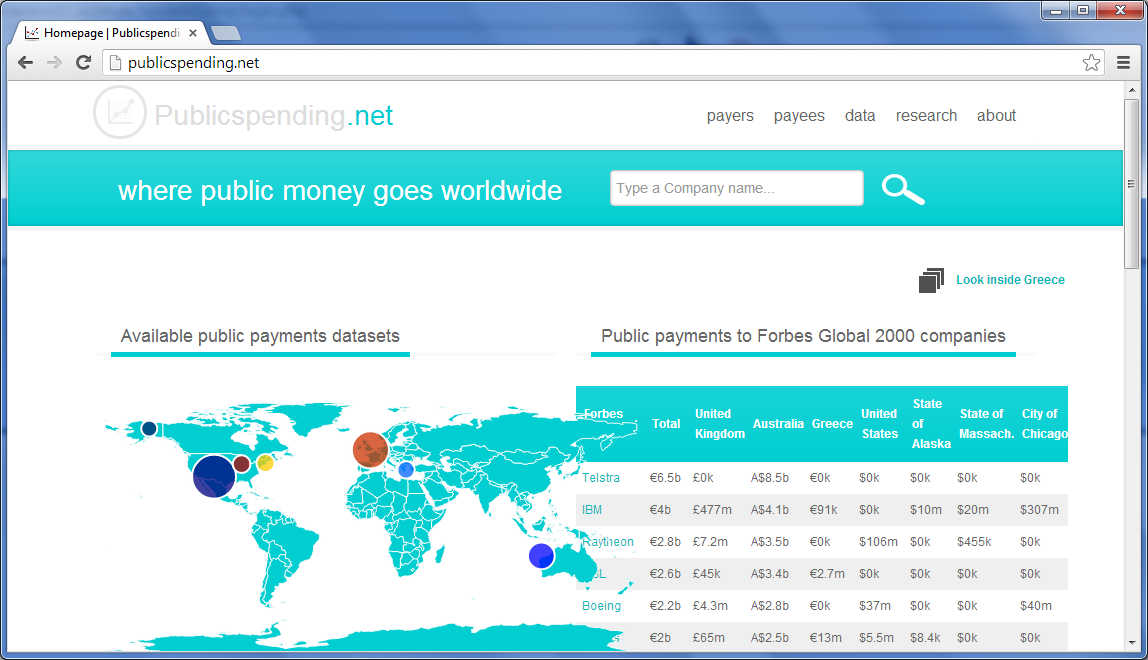
\includegraphics[width=2cm]{imgs/psnet}
\end{figure} & The Public Spending team: \begin{itemize}
                \item Marios Meimaris
                \item Giannis Xidias
                \item Giorgos Vafeiadis
                \item Michalis Klonaras
                \item Panagiotis Kranidiotis
                \item Prodromos Tsiavos
                \item Georgia Lioliou
                \item WWW: \url{http://publicspending.org/}
               \end{itemize}
               
\end{tabular}

\end{table} 


}
  

\frame{
  \frametitle{Roster...} 
  
  \begin{table}[!htb]

\scriptsize
\begin{center}
\begin{tabular}{p{3cm} p{7cm}}
  \begin{figure}[!htb]
\centering
 
\includegraphics[width=1cm]{imgs/chema}
\end{figure} & \begin{itemize}
                \item Dr. Jose María Alvarez-Rodríguez
                \item SEERC (until August, 2013) and Carlos III University of Madrid, Spain
                \item E-mail: \url{josemaria.alvarez@uc3m.es}
                \item WWW: \url{http://www.josemalvarez.es}
               \end{itemize} \\

\begin{figure}[!htb]
\centering
 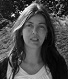
\includegraphics[width=1cm]{imgs/patriop}
\end{figure} & \begin{itemize}
                \item Prof. Dr. Patricia Ordoñez De Pablos
                \item University of Oviedo, Spain
                \item E-mail: \url{patriop@uniovi.es}
               \end{itemize} \\
               

\begin{figure}[!htb]
\centering
 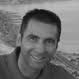
\includegraphics[width=1cm]{imgs/labra}
\end{figure} & \begin{itemize}
                \item Prof. Dr. Jose Emilio Labra-Gayo
                \item University of Oviedo, Spain
                \item E-mail: \url{labra@uniovi.es}
                \item WWW: \url{http://www.di.uniovi.es/~labra}
               \end{itemize}
               \end{tabular}
  \end{center}
\end{table} 

  
}



\appendix



\section*{References}
\bibliographystyle{abbrv}
\tiny
\bibliography{references}


% %%%%%%%%%%%%%%%%%%%%%%%%%%%%%%%%%%%%%%%%%%%%%%%%%%%%%%%%%%%%%%%%%%%%%%

\normalsize

\frame{
\titlepage

}

% %%%%%%%%%%%%%%%%%%%%%%%%%%%%%%%%%%%%%%%%%%%%%%%%%%%%%%%%%%%%%%%%%%%%%%

\end{document}
